\section{Representations through seven elements}\label{sec:small}

DeMeo's small-lattice reduction \cite[Theorem~6.1.1 and Chapter~6]{DeMeo2012}
provides finite-algebra representations for every lattice of at most seven
elements, with one possible exception. We now represent that remaining
lattice directly.  The closure constructions used for the other small
lattices include Snow's parallel-sum construction: take a disjoint union
and add a new bottom and top.  A one-element summand is allowed
\citep[Lemma~3.9]{Snow2000}; in particular, the parallel sum of a
four-element chain and a singleton is represented
\citep[Lemma~4.1]{Snow2000}.

\begin{definition}\label{f:def-l7}
Let $L_7$ have elements $0,1,a,b,c,d,x$, with $0$ least, $1$ greatest, and
with the comparabilities among the five interior elements exactly
\[
 a<c,\qquad b<c,\qquad b<d.
\]
In DeMeo's group-interval labeling these elements are
$J_1,J_2,M_2,M_1,K$, respectively.
\end{definition}

\begin{figure}[htbp]
  \centering
  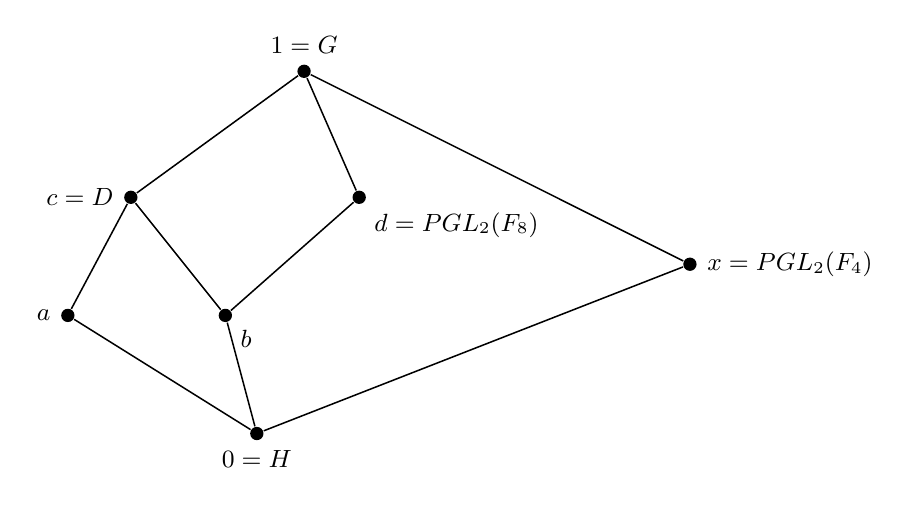
\begin{tikzpicture}[
    x=1cm,y=1cm,
    lattice point/.style={circle,fill,inner sep=1.7pt},
    every label/.style={font=\small},
    line width=0.55pt
  ]
    \node[lattice point,label=below:{$0=H$}] (zero) at (0,0) {};
    \node[lattice point,label=left:{$a$}] (a) at (-2.4,1.5) {};
    \node[lattice point,label=below right:{$b$}] (b) at (-0.4,1.5) {};
    \node[lattice point,label=left:{$c=D$}] (c) at (-1.6,3) {};
    \node[lattice point,label=below right:{$d=\operatorname{PGL}_2(\mathbb F_8)$}]
      (d) at (1.3,3) {};
    \node[lattice point,label=right:{$x=\operatorname{PGL}_2(\mathbb F_4)$}]
      (x) at (5.5,2.15) {};
    \node[lattice point,label=above:{$1=G$}] (one) at (0.6,4.6) {};
    \draw (zero)--(a)--(c)--(one)
          (zero)--(b)--(c)
          (b)--(d)--(one)
          (zero)--(x)--(one);
  \end{tikzpicture}
  \caption{The lattice $L_7$ realized as the subgroup interval $[H,G]$,
    where $G=\operatorname{PGL}_2(\mathbb F_{64})$ and
    $H=\operatorname{PGL}_2(\mathbb F_2)$. The group $D$ is the
    dihedral eigenpair stabilizer of order $126$; its subgroups $a$ and $b$
    containing $H$ have orders $42$ and $18$, respectively. Among the five
    interior elements, the only strict comparabilities are
    $a<c$, $b<c$, and $b<d$.}
  \label{f:fig-l7}
\end{figure}


\begin{proposition}\label{f:prop-l7-interval}
With their usual subfield inclusion, the groups
\[
 H=\operatorname{PGL}_2(\mathbb F_2)
 \le G=\operatorname{PGL}_2(\mathbb F_{64})
\]
have subgroup interval $[H,G]\cong L_7$.
\end{proposition}
\begin{proof}
We first classify the overgroups $H\le K\le G$ by their Sylow
two-subgroups and odd-order eigenpair stabilizers, and then determine
their intersections.
We use the projective-line actions, extending scalars to the algebraic
closure when speaking of eigenlines. For any finite field $Q$, counting
invertible matrices and dividing by scalar matrices gives
\[
 |\operatorname{PGL}_2(Q)|=|Q|(|Q|-1)(|Q|+1).
\]
In particular $|H|=6$ and $H$ induces $S_3$ on its subfield line. It has no
common fixed point: $z\mapsto z+1$ fixes only infinity, and its conjugate by
inversion fixes only zero. Also
\begin{equation}\label{f:eq-centralizer-h}
 C_G(H)=1.
\end{equation}
Indeed, a transformation commuting with these two involutions fixes zero and
infinity individually, so is a scaling; commuting with $z\mapsto z+1$ then
makes that scaling the identity.

Fix an overgroup $H\le K\le G$. In characteristic two, a nonidentity element
of $G$ either has one Jordan block up to scalar, and has order two, or has
two distinct eigenlines, and has odd order. The latter assertion follows by
diagonalizing over a finite extension and taking the ratio of the two
eigenvalues. For each unordered eigenpair, its individual stabilizer in
$K$ is cyclic of odd order, since the diagonal ratio embeds it in the
multiplicative group of a finite field. The nonidentity parts of the
nontrivial such stabilizers partition the nonidentity odd-order elements:
each such element determines its unique eigenpair. Choose representatives
$I_i$ for their $K$-conjugacy classes and put $t_i=|I_i|\ge3$. Their
normalizers stabilize the eigenpairs, so
\[
 |N_K(I_i)|=n_i t_i,\qquad n_i\in\{1,2\}.
\]

The full translation group is a Sylow two-subgroup of $G$, by the order
formula; all Sylow two-subgroups are its conjugates. A Sylow two-subgroup of
$K$ has order $s\ge2$ and hence lies in a translation group, fixing a unique
point of the $\mathbb F_{64}$-line. Distinct Sylow two-subgroups have distinct
fixed points: at any point all involutions fixing it lie in its one
translation group, whose intersection with $K$ is itself a two-group. Let
$\Omega$ be the set of these fixed points. It is a $K$-orbit of size $h>1$,
since otherwise $H$ would fix its unique point.

At a point of $\Omega$, take coordinates putting that point at infinity.
The stabilizer $K_\infty$ is affine. Its translation kernel has order $s$;
its multiplier image has odd order $j$ and preserves the additive subgroup
of translation parameters. Nonidentity multipliers act freely on nonzero
parameters, so $j\mid s-1$. Therefore $|K|=hsj$, and the number of involutions
is $h(s-1)$. Counting the identity, the involutions, and the odd-order
elements yields
\begin{equation}\label{f:eq-overgroup-count}
 \sum_i\frac1{n_i}\left(1-\frac1{t_i}\right)
 =1-\frac{s-1}{sj}-\frac1{hsj}
 =1-\frac1j+\frac{h-1}{hsj}.
\end{equation}
The sum is nonempty because $H$ contains an element of order three.

\emph{The case $j=1$.}
The right side of \Cref{f:eq-overgroup-count} is less than $1/s$; each
summand is at least $1/3$. Thus $s=2$, and there is exactly one summand. It
must have $n_i=2$, because a summand with $n_i=1$ is at least $2/3$.
Substitution gives $t_i=h$, so
$|N_K(I_i)|=2h=|K|$. Hence $K$ lies in the setwise stabilizer of one eigenpair.
The order-three subgroup of $H$ must fix the pair individually, since it
cannot act nontrivially on two points. This eigenpair is therefore the one
of that order-three subgroup.

\emph{The case $j>1$.}
Now $s\ge4$. The number $j$ is one of the $t_i$: a generator of the multiplier
image lifts to an affine map with nonidentity multiplier, two fixed points,
and order $j$. The individual stabilizer of its two fixed points embeds in
the multiplier image and contains that cyclic subgroup, so has order $j$.
If the sum in \Cref{f:eq-overgroup-count} had only this term, it would be at
most $1-1/j$, contrary to the equation. The whole sum is less than $1$.
Since each summand is at least $1/3$, there are exactly two summands, and
both have $n_i=2$; otherwise their sum would be at least $2/3+1/3$.
Writing $t$ for the other order gives
\begin{equation}\label{f:eq-overgroup-parameters}
 1-\frac jt=\frac{2(h-1)}{hs}.
\end{equation}
In particular $t>j$, and $s(t-j)<2t$ implies
\[
 0<t-j<\frac{2j}{s-2}\le\frac{2(s-1)}{s-2}\le3.
\]
The two orders are odd, so $t=j+2$. Equation
\eqref{f:eq-overgroup-parameters} now gives $h(j+2-s)=j+2$.
Since $h>0$, we have $j>s-2$, and $j\le s-1$ therefore forces
$j=s-1$ and $h=s+1$.

The multiplier realization gives $s-1\mid63$. As $s$ is a power of two with
$4\le s\le64$, it follows that $s\in\{4,8,64\}$. The multiplier group is
then exactly $\mathbb F_s^\times$ inside $\mathbb F_{64}^\times$. The
translation-parameter subgroup, of size $s$, is stable under these scalars,
so is a one-dimensional $\mathbb F_s$-space, say $v\mathbb F_s$. Translations
act freely on the other $s$ points of $\Omega$, and hence those points form
one coset of $v\mathbb F_s$. An affine coordinate change thus makes
$\Omega=\mathbb P^1(\mathbb F_s)$.

Its full setwise stabilizer in $G$ is $\operatorname{PGL}_2(\mathbb F_s)$:
the images of infinity, zero, and one determine a projective transformation,
and every ordered triple of distinct subfield points is the image of that
triple under a subfield transformation. The equality
$|K|=(s+1)s(s-1)$ now gives
$K=g\operatorname{PGL}_2(\mathbb F_s)g^{-1}$ for some $g\in G$.
This conjugate is in fact the standard subfield group. Let $\sigma$ be the
entrywise $s$-power automorphism. It fixes both $H$ and $g^{-1}Hg$ pointwise.
Consequently $g\sigma(g^{-1})$ centralizes $H$, so
\Cref{f:eq-centralizer-h} gives $\sigma(g)=g$ in the projective group.
Normalize one nonzero matrix entry of a representative of $g$ to $1$;
all its entries are then fixed by $\sigma$. Thus
$g\in\operatorname{PGL}_2(\mathbb F_s)$, as required.

It remains to record the incidences between the groups in this list. The
eigenpair of the order-three subgroup of $H$ splits over $\mathbb F_{64}$.
Its full setwise stabilizer $D$ is dihedral of order $2\cdot63$ and contains
$H$, generated there by a rotation of order three and a flip. Subgroups
between $H$ and $D$ correspond to rotation subgroups containing the
order-three one, after adjoining that same flip. Their orders are
$6,18,42,126$, so there are precisely two strict intermediate groups, of
orders $18$ and $42$.

The other proper overgroups are the standard subfield groups over
$\mathbb F_8$ and $\mathbb F_4$, whose intersection is $H$: normalize one nonzero matrix entry to $1$
and use $\mathbb F_8\cap\mathbb F_4=\mathbb F_2$. Over
$\mathbb F_4$ the eigenpair is split, so its setwise stabilizer has order
$2(4-1)=6$; consequently
$D\cap\operatorname{PGL}_2(\mathbb F_4)=H$. Over $\mathbb F_8$ the pair is
nonsplit, because $3\nmid7$. Its individual stabilizer has order $8+1=9$.
To see the latter count directly, matrices fixing the two eigenlines
centralize a matrix with irreducible quadratic minimal polynomial. Its
invertible centralizer is the multiplicative group of the quadratic field
extension, and quotienting by subfield scalars gives order
$(8^2-1)/(8-1)=9$. The flip from $H$ doubles this order. Hence
$D\cap\operatorname{PGL}_2(\mathbb F_8)$ is exactly the order-$18$ group.
We obtain the asserted interval by taking
\[
 c=D,\quad d=\operatorname{PGL}_2(\mathbb F_8),\quad
 x=\operatorname{PGL}_2(\mathbb F_4),
\]
and taking $a,b$ to be the groups of orders $42,18$, respectively.
\end{proof}

\begin{lemma}[Coset-action correspondence]\label{f:lem-coset}
For finite groups $H\le G$, the full congruence lattice of the unary algebra
given by the left $G$-action on $G/H$ is isomorphic to $[H,G]$.
\end{lemma}
\begin{proof}
For a $G$-invariant equivalence $\theta$ on $G/H$, put
$K_\theta=\{g\in G:gH\mathrel\theta H\}$. This contains $H$. If
$g,g'\in K_\theta$, invariance applied to $gH\mathrel\theta g'H$ gives
$H\mathrel\theta g^{-1}g'H$, so $K_\theta$ is a subgroup. Conversely,
$H\le K\le G$ gives the invariant equivalence obtained by pulling equality
back along $G/H\to G/K$. These constructions are inverse and preserve order.
\end{proof}

\begin{theorem}\label{f:small-lattices}
Every finite nonempty lattice of at most seven elements is representable.
\end{theorem}
\begin{proof}
\Cref{f:prop-l7-interval,f:lem-coset} represent $L_7$ by a finite unary
algebra. DeMeo's small-lattice reduction supplies the other lattices
\cite[Theorem~6.1.1]{DeMeo2012}.
\end{proof}
